\documentclass[11pt,a4paper,twocolumn]{article}

% === Core Packages ===
\usepackage[margin=2cm]{geometry}
\usepackage[utf8]{inputenc}
\usepackage[T1]{fontenc}
\usepackage{times}
\usepackage{amsmath,amssymb}
\usepackage{graphicx}
\usepackage{booktabs}
\usepackage{float}
\usepackage{enumitem}
\usepackage{tikz}
\usepackage{pgfplots}
\pgfplotsset{compat=1.18}
\usetikzlibrary{arrows.meta,shapes.geometric,positioning,calc,decorations.markings,fit,backgrounds}

% === Citation (IEEE style) ===
\usepackage[numbers,sort&compress]{natbib}
\bibliographystyle{IEEEtranN}

% === Hyperref ===
\usepackage[hidelinks]{hyperref}
\usepackage{xurl}

% === Settings ===
\setlength{\parindent}{1em}
\setlength{\parskip}{0.3em}

% === PDF metadata ===
\hypersetup{
  pdftitle={Red de Reputación Descentralizada: Un marco para la organización natural de la sociedad},
  pdfauthor={Pavel Kudrna},
  pdfsubject={Personix — a decentralized reputation network},
  pdfkeywords={Personix, decentralized reputation, reputation social network,
    decentralized identifiers, DID, meritocracy, censorship resistance},
}

% === Title ===
\title{\textbf{Red de Reputación Descentralizada:\\Un marco para la organización natural de la sociedad}}
\author{Pavel Kudrna\\Personix Project --- \url{https://personix.org}\\Prague, Czechia\\Draft v1 --- March 2026}
\date{}

\begin{document}
\maketitle

% ============================================================
% ABSTRACT
% ============================================================
\begin{abstract}
El sentido de justicia---la convicción de que las injusticias se reparan y el mérito se recompensa---es la fuerza cohesiva más poderosa de la sociedad. Cuando las instituciones centralizadas de gobierno no pueden brindar este sentido porque el coste de hacer valer un derecho supera el valor del propio derecho, la cohesión social se erosiona. Las estructuras institucionales actuales no logran resolver una clase significativa de disputas de la misma manera sistemática en que la planificación central falla al asignar recursos: mediante la asimetría de información, la ausencia de bucles de retroalimentación y la desconexión de quienes toman decisiones respecto de las consecuencias de esas decisiones. Este artículo presenta una Red Social de Reputación (RSN): una capa de comunicación descentralizada, incorruptible y resistente a la censura, construida sobre Identificadores Descentralizados (DID), que permite a participantes seudónimos publicar, verificar y consumir información de reputación sobre el comportamiento en el mundo real. El mecanismo central se sustenta en tres principios de diseño: (1)~una estructura de costes asimétrica en la que leer datos de reputación es barato pero escribir requiere un esfuerzo verificable; (2)~un protocolo de selección de verificadores no determinista basado en hashing consistente que pone precio a las afirmaciones radicales mediante costes de iteración crecientes; y (3)~un modelo de autoridad de reputación impulsado por el mercado en el que verificadores privados arriesgan su reputación acumulada sobre la exactitud de las afirmaciones que respaldan. La arquitectura resultante produce una meritocracia emergente sin coordinación central y habilita una ruta de migración gradual y reversible desde los sistemas administrados por el Estado actuales.
\end{abstract}

% ============================================================
% 1. INTRODUCTION
% ============================================================
\section{Introducción}

\subsection{El problema de la confianza centralizada}

El gobierno moderno se apoya en una suposición fundamental: que las instituciones centralizadas pueden mediar la confianza entre desconocidos a gran escala. Los tribunales dirimen disputas. Los registros certifican la propiedad. Los organismos reguladores hacen cumplir las normas. Estas instituciones se diseñaron en una época en la que la información era escasa, la comunicación era lenta y delegar la autoridad en un órgano central era el único mecanismo de coordinación viable. El gobierno centralizado, sin embargo, fracasa por las mismas razones estructurales que la planificación central: asimetría de información, ausencia de bucles de retroalimentación y desconexión de quienes toman decisiones respecto de las consecuencias de esas decisiones.

La suposición fracasa, por ejemplo, cuando el coste de la mediación institucional supera el valor de la disputa. Considérese a un inquilino que descubre que su apartamento alquilado carece de un certificado de seguridad eléctrica exigido por ley---una condición que supone un peligro inmediato para la vida. El derecho legal del inquilino a rescindir el contrato es inequívoco. Sin embargo, el coste de hacer valer ese derecho a través del sistema judicial supera el valor monetario de la fianza y los daños adeudados, incluso incluyendo una posible indemnización legal~\cite{czcourtfees}. La respuesta racional es asumir la pérdida y salir.

No se trata de un caso límite patológico. Es la experiencia habitual para una clase significativa de disputas en las que el daño es real pero lo que está en juego económicamente cae por debajo del umbral a partir del cual la ejecución institucional se vuelve económicamente racional. El resultado es un sistema que favorece estructuralmente a los malos actores: quienes perjudican a otros en volúmenes por debajo de este umbral pueden actuar con impunidad, porque el coste de buscar justicia recae sobre la parte perjudicada.

El ejemplo anterior está tomado del entorno jurídico del autor---el sistema de derecho civil checo. En otras tradiciones jurídicas---el common law basado en precedentes, el derecho consuetudinario, los sistemas mixtos---la justicia falla de maneras y en grados distintos, según las particularidades culturales y procesales de cada jurisdicción. Es probable que los lectores reconozcan ejemplos equivalentes en su propio contexto. Lo que es estructuralmente universal es el patrón: las disputas cuyo valor cae por debajo del umbral de la ejecución económicamente racional terminan con la pérdida absorbida por la parte perjudicada. La RSN no promete una justicia perfecta---simplemente reduce la ventaja estructural de la que disfrutan los malos actores cuando la ejecución institucional resulta antieconómica.

\subsection{Por qué las soluciones existentes se quedan cortas}

\textbf{Los marcos de identidad descentralizada (DID)}~\cite{did2022} proporcionan mecanismos criptográficos para la gestión de identidad autosoberana, pero se centran principalmente en la verificación de identidad sin abordar la cuestión más amplia de la reputación conductual.

\textbf{Los Soulbound Tokens (SBT)}~\cite{weyl2022} capturan la idea de que la reputación es no transferible, pero dependen de una infraestructura de cadena de bloques con limitaciones de escalabilidad y no abordan los incentivos económicos que rigen la entrada de información. Conceptos relacionados como los tokens de mérito (por ejemplo, Liberland) comparten una filosofía similar, pero siguen atados a marcos jurisdiccionales concretos.

\textbf{Las Organizaciones Autónomas Descentralizadas (DAO)}~\cite{buterin2014} implementan la gobernanza mediante contratos inteligentes, pero replican dinámicas plutocráticas en las que la influencia es proporcional al capital. La votación cuadrática~\cite{buterin2019} lo mitiga en parte pero limita su adopción práctica. Las DAO también se enfrentan al \emph{problema del oráculo} fundamental: los contratos inteligentes no pueden verificar de forma fiable estados del mundo real sin una fuente externa de confianza, y este problema no tiene solución general dentro de la arquitectura de cadena de bloques.

Ningún sistema existente combina descentralización, resistencia a la censura, seudonimia, coste de entrada verificable y consenso emergente.

\subsection{Aportaciones}

Este artículo realiza las siguientes aportaciones:
\begin{enumerate}[nosep]
\item La definición de la \textbf{Red Social de Reputación (RSN)}, un protocolo descentralizado que extiende el marco DID para admitir el intercambio bilateral de reputación.
\item Un \textbf{protocolo de selección de verificadores no determinista} basado en hashing consistente~\cite{karger1997}.
\item El \textbf{Principio del Radicalismo Costoso}, que pone precio a las afirmaciones según su distancia respecto del consenso de la red mediante tres canales de coste que se acumulan.
\item Un \textbf{modelo de Autoridad Reputable} con incentivos asimétricos en el que un respaldo falso cuesta catastróficamente más que las tarifas legítimas.
\item Una \textbf{ruta de migración gradual} a través de una infraestructura fiscal paralela.
\end{enumerate}

% ============================================================
% 2. DESIGN PRINCIPLES
% ============================================================
\section{Principios de diseño}

La arquitectura de la RSN está condicionada por cinco principios de diseño innegociables.

\textbf{Continuidad y evolución.} El sistema coexiste con las instituciones existentes durante un periodo de transición de duración indefinida. La transición debe ser reversible en cada etapa.

\textbf{Voluntariedad y responsabilidad.} La participación es voluntaria, pero la voluntariedad va unida a la responsabilidad: un participante que asume el control de una función institucional asume simultáneamente las obligaciones que la acompañan.

\textbf{Diversidad y neutralidad cultural.} El consenso surge de las interacciones bilaterales, no de reglas predefinidas impuestas por los diseñadores del sistema.

\textbf{Resiliencia y resistencia a la censura.} El coste de censurar la red debe superar el coste de tolerarla. Solo un totalitarismo total---a un coste político y económico ruinoso---puede suprimir el sistema.

\textbf{Consenso y ejecución.} El sistema incorpora las tendencias humanas hacia la mezquindad, el rencor y la satisfacción retributiva como características estructurales. La mala conducta no se prohíbe; se pone a precio.

% ============================================================
% 3. SYSTEM OVERVIEW
% ============================================================
\section{Visión general del sistema}

\subsection{Red Social de Reputación}

La RSN es una capa de comunicación descentralizada, entre pares, en la que los participantes intercambian información verificable sobre el comportamiento en el mundo real. Sus propiedades definitorias son: infraestructura descentralizada e incensurable; participación seudónima mediante DID; estructura de costes asimétrica (leer es barato, escribir es caro); verificabilidad criptográfica; y \textbf{soporte de estándares}---formatos legibles por máquina para la información propagada por la red, para los servicios ofrecidos por las autoridades (composición de afirmaciones, respaldo, servicio de testigo) y para el formato de política, incluidas las reglas para evaluar la reputación de la contraparte y valorar el riesgo de discrepancia de política (entre el comportamiento declarado y el real).

\subsection{Componentes arquitectónicos}

La RSN consta de cuatro componentes principales (Fig.~\ref{fig:architecture}):
\begin{enumerate}[nosep]
\item \textbf{Capa DID.} Identidades de los participantes con reglas declaradas, metadatos de reputación y enrutamiento de red.
\item \textbf{Protocolo de afirmaciones.} Formato estructurado para publicar aserciones sobre eventos del mundo real.
\item \textbf{Red de verificación.} Protocolo descentralizado para asignar verificadores mediante hashing consistente.
\item \textbf{Capa de agregación de reputación.} Servicios que producen resúmenes de reputación legibles por humanos.
\end{enumerate}

\begin{figure}[ht]
\centering
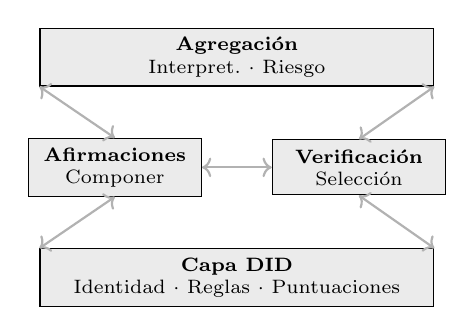
\begin{tikzpicture}[
    layer/.style={draw, minimum height=0.7cm, align=center, font=\scriptsize, fill=black!8},
    arr/.style={<->, thick, gray!60}
]
\node[layer, minimum width=5cm] (agg) at (0,2.8) {\textbf{Agregación}\\Interpret.\ $\cdot$ Riesgo};
\node[layer, minimum width=2.2cm] (claim) at (-1.55,1.4) {\textbf{Afirmaciones}\\Componer};
\node[layer, minimum width=2.2cm] (verif) at (1.55,1.4) {\textbf{Verificación}\\Selección};
\node[layer, minimum width=5cm] (did) at (0,0) {\textbf{Capa DID}\\Identidad $\cdot$ Reglas $\cdot$ Puntuaciones};

\draw[arr] (agg.south west) -- (claim.north);
\draw[arr] (agg.south east) -- (verif.north);
\draw[arr] (claim.east) -- (verif.west);
\draw[arr] (claim.south) -- (did.north west);
\draw[arr] (verif.south) -- (did.north east);
\end{tikzpicture}
\caption{Arquitectura de cuatro capas de la RSN.}
\label{fig:architecture}
\end{figure}

\subsection{Roles de los participantes}

Una transacción de verificación implica hasta seis roles DID distintos (Fig.~\ref{fig:roles}): \textbf{Emisor} ($DID_I$, crea y envía la afirmación), \textbf{Sujeto} ($DID_S$, el DID sobre el que trata la afirmación---puede coincidir con el Emisor), \textbf{Autoridad} ($DID_A$, respalda la afirmación por una tarifa; también puede ofrecer servicios de testigo---\emph{opcional}), \textbf{Testigo} ($DID_{W_{1..n}}$, supervisor de incógnito de la honestidad del verificador mediante códigos de reto---\emph{opcional}), \textbf{Verificador} ($DID_V$, seleccionado algorítmicamente para publicar la afirmación) y la \textbf{RSN} (la red donde se publican las afirmaciones verificadas). Cualquier rol puede delegarse en otro DID (Sección~7.4). Una Autoridad suele combinar el respaldo con servicios de testigo, pero ambas funciones son lógicamente independientes.

\begin{figure}[ht]
\centering
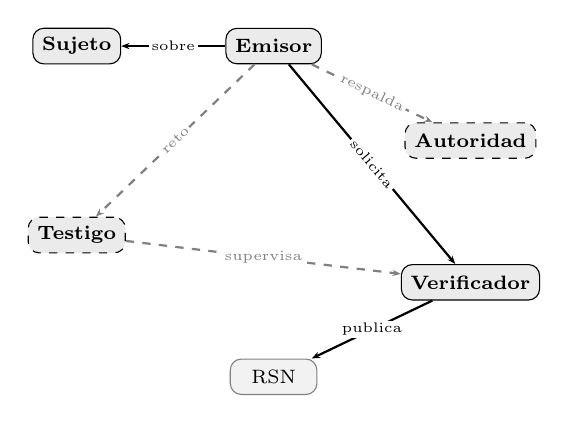
\begin{tikzpicture}[
    role/.style={draw, rounded corners, minimum width=1.1cm, minimum height=0.45cm, align=center, font=\scriptsize, fill=black!8},
    opt/.style={draw, rounded corners, minimum width=1.1cm, minimum height=0.45cm, align=center, font=\scriptsize, fill=black!8, dashed},
    arr/.style={-{Stealth[length=3pt]}, thick},
    oarr/.style={-{Stealth[length=3pt]}, thick, dashed, gray},
    lbl/.style={font=\tiny, fill=white, inner sep=1pt}
]
\node[role] (I) at (0,2.4) {\textbf{Emisor}};
\node[role] (S) at (-2.5,2.4) {\textbf{Sujeto}};
\node[opt] (A) at (2.5,1.2) {\textbf{Autoridad}};
\node[opt] (W) at (-2.5,0) {\textbf{Testigo}};
\node[role] (V) at (2.5,-0.6) {\textbf{Verificador}};
\node[role, fill=black!5, draw=gray] (N) at (0,-1.8) {RSN};

\draw[arr] (I) -- node[lbl] {sobre} (S);
\draw[oarr] (I) -- node[lbl,sloped] {respalda} (A);
\draw[oarr] (I) -- node[lbl,sloped] {reto} (W);
\draw[arr] (I) -- node[lbl,sloped] {solicita} (V);
\draw[oarr] (W) -- node[lbl] {supervisa} (V);
\draw[arr] (V) -- node[lbl] {publica} (N);
\end{tikzpicture}
\caption{Roles DID en una transacción de verificación. Discontinuo = opcional (Autoridad, Testigo).}
\label{fig:roles}
\end{figure}

\subsection{Incorruptibilidad: cuatro fuerzas}

La incorruptibilidad de la RSN no surge de un único mecanismo, sino de cuatro fuerzas concurrentes. Ninguna es suficiente por sí sola; solo su combinación hace que un intento de corrupción sea económicamente irracional.

\textbf{Objetivo impredecible.} El verificador de cada afirmación se selecciona de forma no determinista mediante hashing consistente (Sección~5.3). Un atacante no puede fijar de antemano un verificador concreto para sobornarlo, porque la identidad del verificador es función del contenido de la afirmación y de las iteraciones previas, no de la elección del emisor.

\textbf{Apalancamiento reputacional---sube despacio, cae rápido.} La reputación solo puede ganarse de forma incremental, mediante un comportamiento consistente sostenido. Sin embargo, puede perderse de manera catastrófica en un único respaldo fraudulento (Sección~6.2). Esta asimetría implica que años de reputación acumulada pueden destruirse con un solo respaldo deshonesto; la estrategia óptima sigue siendo rechazar las afirmaciones sospechosas.

\textbf{Promesa pública.} Cada Titular de un DID declara públicamente su política---un conjunto de reglas legible por máquina que se compromete a cumplir. La divergencia entre la declaración y el comportamiento real es detectable y se pone a precio como una infracción reputacional más grave que la violación subyacente (Sección~7.3). La hipocresía es, por tanto, más costosa que la deshonestidad directa.

\textbf{Asimetría de coste de ataque en malla.} El coste de censurar o desestabilizar la red crece de forma no lineal con el tamaño y la densidad de la red, mientras que el coste de tolerarla permanece constante. Para que la censura resulte rentable, un actor centralizado tendría que aplicarla a toda la red---exigiendo medidas desproporcionadas frente a cualquier beneficio concebible (Sección~10).

% ============================================================
% 4. DECENTRALIZED IDENTITY MODEL
% ============================================================
\section{Modelo de identidad descentralizada}

\subsection{DID con propiedades especiales}

La RSN extiende la especificación W3C DID Core~\cite{did2022} con: \textbf{Reglas Declaradas} (compromisos conductuales legibles por máquina), \textbf{Metadatos de Reputación} (puntuación conductual agregada) y \textbf{Enrutamiento de Red} (pasarela onion mutable, separada de la posición estable en el anillo).

\subsection{Ciclo de vida de una afirmación}

Una afirmación transita por seis etapas (Fig.~\ref{fig:lifecycle}): composición, respaldo opcional por una autoridad, selección de verificador mediante hashing consistente, decisión de verificación (aceptar o rechazar con iteración), publicación y actualización de reputación para todas las partes.

\begin{figure}[ht]
\centering
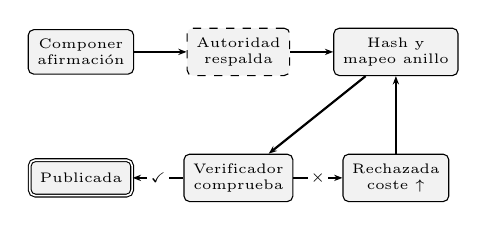
\begin{tikzpicture}[
    stp/.style={draw, rounded corners=2pt, minimum width=1.3cm, minimum height=0.45cm, align=center, font=\tiny, fill=black!5},
    arr/.style={-{Stealth[length=3pt]}, thick},
    lbl/.style={font=\tiny, fill=white, inner sep=1pt}
]
\node[stp] (comp) at (0,0) {Componer\\afirmación};
\node[stp, dashed] (auth) at (2.0,0) {Autoridad\\respalda};
\node[stp] (hash) at (4.0,0) {Hash y\\mapeo anillo};
\node[stp] (ver) at (2.0,-1.6) {Verificador\\comprueba};
\node[stp, double] (pub) at (0,-1.6) {Publicada};
\node[stp] (rej) at (4.0,-1.6) {Rechazada\\coste $\uparrow$};

\draw[arr] (comp) -- (auth);
\draw[arr] (auth) -- (hash);
\draw[arr] (hash) -- (ver);
\draw[arr] (ver) -- node[lbl] {\checkmark} (pub);
\draw[arr] (ver) -- node[lbl] {$\times$} (rej);
\draw[arr] (rej) -- ++(0,0.8) -| (hash);
\end{tikzpicture}
\caption{Ciclo de vida de una afirmación con bucle de iteración.}
\label{fig:lifecycle}
\end{figure}

\subsection{Relación con W3C DID Core}

El modelo de identidad de la RSN es un superconjunto propio de la especificación W3C DID Core~\cite{did2022}. Todos los DID de la RSN son DID válidos de W3C. Las extensiones específicas de la RSN se codifican como propiedades del documento DID definidas en una especificación de método DID dedicada, compatible con infraestructura existente como ION~\cite{buchner2021} y Ceramic~\cite{ceramic2023}.

% ============================================================
% 5. VERIFICATION AND PROPAGATION
% ============================================================
\section{Verificación y propagación de la información}

\subsection{Coste de la entrada de información}

El principio económico central de la RSN es la asimetría entre leer y escribir. Leer datos de reputación se aproxima a un coste marginal nulo para los participantes que forman parte de la red DID y tienen un acceso acorde con su reputación---los recién llegados deben ganar progresivamente un acceso más amplio (véase anti-parasitismo). Escribir---entendido como la materialización duradera de la reputación en la red, no como un acto técnico puntual---requiere una inversión acumulada verificable en tres dimensiones: \textbf{tiempo} (años de vida dedicados a un comportamiento consistente, compromisos cumplidos y relaciones cultivadas), \textbf{energía} (esfuerzo invertido en un trato honesto, cuidado de las asociaciones y fiabilidad a largo plazo) y \textbf{dinero} (inversión en el propio nombre---desarrollo profesional, calidad del propio trabajo, restitución por los daños causados). La reputación no puede comprarse al instante---es el resultado de una acumulación de toda una vida que el sistema simplemente hace visible y transferible entre contextos. Los costes técnicos puntuales del protocolo (firmas criptográficas, tarifas de verificador) son insignificantes en comparación con esta inversión subyacente.

\subsection{Grafo social y profundidad de contactos}

La RSN es fundamentalmente una red social: cada DID añade contactos (otros DID) que permiten la conexión. Estos contactos tienen sus propios contactos, y así sucesivamente. La búsqueda algorítmica de verificadores opera dentro de una profundidad configurable $h$ de contactos enlazados (por ejemplo, $h=3$: los contactos directos, sus contactos y los contactos de los contactos). Esta arquitectura no requiere una única cadena de bloques global---favorece de forma natural la aparición de comunidades/agrupaciones con solapamientos hacia otras comunidades. Todo participante DID debe tener una \textbf{política} publicada---un conjunto de reglas legible por máquina que rige cómo se evalúan las solicitudes entrantes. Las violaciones de política se registran en la red como artefactos negativos.

\subsection{Selección algorítmica de verificadores}

El protocolo de verificación emplea hashing consistente~\cite{karger1997} (Fig.~\ref{fig:verifier}). La verificación es un servicio de pago: los verificadores operan por una tarifa, creando un mercado donde la competencia impulsa el precio, la velocidad y la fiabilidad.

\textbf{Paso 1.} El documento de la afirmación se concatena con el resultado del hash de la iteración anterior (o $\varnothing$ en la primera iteración) y se somete a hash:
\begin{equation}
\text{pos} = f_h(\text{claim} \| \text{prev\_hash})
\label{eq:hash}
\end{equation}

El algoritmo debe incluir la \emph{ruta completa} de todas las solicitudes y respuestas previas---no meramente un hash de la iteración anterior. La respuesta completa de cada verificador (aceptación, rechazo, precio cotizado, motivo) se añade al documento en crecimiento, verificable mediante firmas criptográficas en cada paso.

\textbf{Paso 2.} El hash se mapea a $N$ posiciones en el anillo de hashing consistente, distribuidas uniformemente (por ejemplo, para $N=4$: $+0^{\circ}, +90^{\circ}, +180^{\circ}, +270^{\circ}$). Desde cada posición, una búsqueda en sentido horario selecciona el DID más cercano como candidato a verificador (Fig.~\ref{fig:multipoint}). $N$ es un parámetro variable que puede depender del porcentaje de DID actualmente activos, de la hora del día o de la capacidad de respuesta histórica de la red.

\textbf{Paso 3.} El Verificador acepta (publica, arriesgando reputación) o rechaza (volviendo al Paso~1 con el hash del rechazo). Cuando un nodo no responde pese a declararse en línea, la siguiente solicitud debe incluir todas las respuestas de los $N$ candidatos a verificador anteriores.

\textbf{Anti-parasitismo.} Los DID objetivo pueden fijar tarifas o restricciones de acceso para las consultas de DID nuevos con poca reputación. Este mecanismo graduado (no binario) obliga a los recién llegados a construir reputación mediante actividad genuina antes de consumir libremente los datos de otros.

\begin{figure}[ht]
\centering
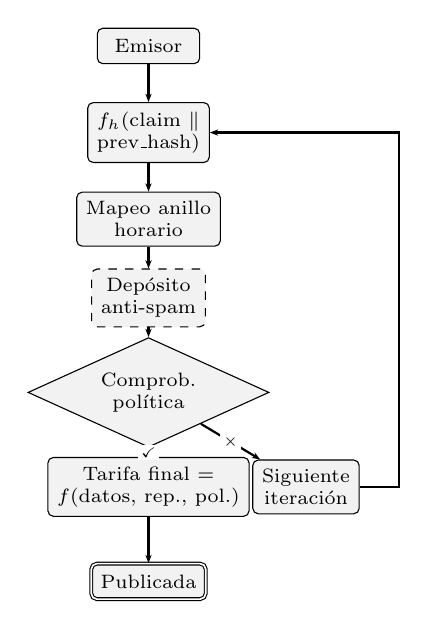
\begin{tikzpicture}[
    box/.style={draw, rounded corners=2pt, minimum width=1.3cm, minimum height=0.45cm, align=center, font=\scriptsize, fill=black!5},
    dec/.style={draw, diamond, aspect=2.2, minimum width=0.9cm, align=center, font=\scriptsize, fill=black!5},
    arr/.style={-{Stealth[length=3pt]}, thick},
    lbl/.style={font=\tiny, fill=white, inner sep=1pt}
]
\node[box] (iss) at (0,0) {Emisor};
\node[box] (hash) at (0,-1.1) {$f_h$(claim $\|$\\prev\_hash)};
\node[box] (ring) at (0,-2.2) {Mapeo anillo\\horario};
\node[box, dashed] (spam) at (0,-3.2) {Depósito\\anti-spam};
\node[dec] (check) at (0,-4.4) {Comprob.\\política};
\node[box] (rej) at (2,-5.6) {Siguiente\\iteración};
\node[box] (fee) at (0,-5.6) {Tarifa final =\\$f$(datos, rep., pol.)};
\node[box, double] (pub) at (0,-6.8) {Publicada};

\draw[arr] (iss) -- (hash);
\draw[arr] (hash) -- (ring);
\draw[arr] (ring) -- (spam);
\draw[arr] (spam) -- (check);
\draw[arr] (check) -- node[lbl] {$\times$} (rej);
\draw[arr] (check) -- node[lbl] {\checkmark} (fee);
\draw[arr] (fee) -- (pub);
\draw[arr] (rej.east) -- ++(0.5,0) |- (hash.east);
\end{tikzpicture}
\caption{Protocolo de selección de verificadores. El depósito anti-spam es opcional y puede ser reembolsable. La tarifa final solo se paga en caso de aceptación.}
\label{fig:verifier}
\end{figure}

Cada rechazo añade la respuesta completa del verificador (incluidos motivos y condiciones) al documento de la afirmación, ampliando su contenido. A partir del documento ampliado se calcula de forma no determinista un nuevo hash, que se mapea a una posición diferente del anillo y selecciona un verificador distinto. La documentación de la ruta completa es obligatoria---el emisor no puede predecir ni influir en el siguiente verificador. Si un verificador ignora una solicitud pese a tener una política declarada compatible, los testigos (si están presentes) lo registran, y el emisor puede adjuntar la prueba del testigo en la publicación final.

\begin{figure}[ht]
\centering
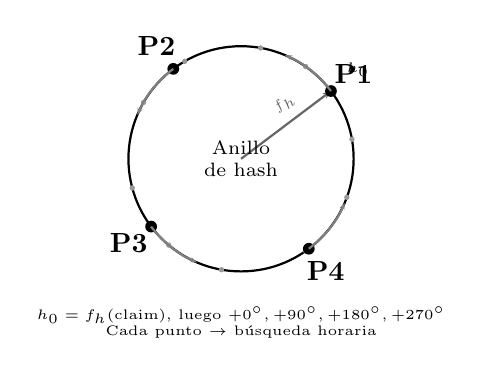
\begin{tikzpicture}[scale=0.65]
% Ring
\draw[thick] (0,0) circle (2.2cm);
% DID nodes on ring
\foreach \a in {10,55,80,120,150,195,230,260,305,340} {
  \fill[black!40] (\a:2.2) circle (1.5pt);
}
% Hash offset arrow pointing to initial position
\draw[-{Stealth[length=3pt]}, thick, black!60] (0,0) -- node[font=\tiny,above,sloped,pos=0.6] {$f_h$} (37:2.2);
\fill[black] (37:2.2) circle (2pt);
\node[font=\tiny,anchor=south west] at (37:2.35) {$h_0$};
% N=4 points offset from h0 by +0, +90, +180, +270
\foreach \offset/\l in {0/P1,90/P2,180/P3,270/P4} {
  \pgfmathsetmacro{\ang}{37+\offset}
  \node[fill=black, circle, inner sep=1.5pt] (p\offset) at (\ang:2.2) {};
  \node[font=\tiny,font=\bfseries] at (\ang:2.75) {\l};
  % clockwise search arc
  \draw[-{Stealth[length=2.5pt]}, thick, gray] (\ang:2.2) arc (\ang:\ang+30:2.2);
}
\node[font=\scriptsize, align=center] at (0,0) {Anillo\\de hash};
\node[font=\tiny, align=center] at (0,-3.2) {$h_0 = f_h(\text{claim})$, luego $+0^{\circ},+90^{\circ},+180^{\circ},+270^{\circ}$\\Cada punto $\rightarrow$ búsqueda horaria};
\end{tikzpicture}
\caption{Selección multipunto ($N{=}4$). El hash $h_0$ fija el desplazamiento; 4 puntos distribuidos uniformemente desde $h_0$.}
\label{fig:multipoint}
\end{figure}

\subsection{Protocolo de testigos}

El rol de \textbf{Testigo} proporciona rendición de cuentas de incógnito sobre la honestidad del verificador mediante un protocolo criptográfico de códigos de reto:

\textbf{Paso W1.} El solicitante firma la solicitud de verificación y la envía a $N_w$ testigos---contactos de la red social del solicitante, o proveedores especializados de servicios de testigo que operan por una tarifa.

\textbf{Paso W2.} Cada testigo $w_i$ firma toda la solicitud firmada, conserva la firma original $\sigma_i$ y calcula un código de reto $c_i = h(\sigma_i)$. El código de reto se añade a la solicitud.

\textbf{Paso W3.} La solicitud, que ahora lleva $N_w$ códigos de reto, se envía al verificador. El verificador observa los códigos pero \emph{no puede determinar} quiénes son los testigos ni si los códigos corresponden a firmas reales.

\textbf{Paso W4 (verificador honesto).} Si el verificador responde conforme a su política declarada, los códigos de reto permanecen opacos. Los testigos nunca se revelan. No se publica ningún dato adicional.

\textbf{Paso W5 (violación de política).} Si el verificador viola su política (ignora la solicitud, responde de forma incoherente), el solicitante conserva las firmas originales $\sigma_i$ de los testigos. Estas pueden publicarse como datos acompañantes: cualquiera puede verificar $c_i = h(\sigma_i)$, demostrando que el testigo estaba presente. El solicitante puede publicar de forma independiente---el verificador ya firmó los códigos de reto en su respuesta.

\textbf{La propiedad del farol.} El solicitante puede sustituir algunos o todos los códigos de reto por valores aleatorios. El verificador no puede distinguir los códigos genuinos (respaldados por autoridades de alta reputación) del ruido. Esta \emph{incertidumbre} es el mecanismo de ejecución: cada solicitud lleva el riesgo de que una autoridad respetada esté observando de incógnito. El coste de mantener esta presión es casi nulo (generar números aleatorios), mientras que el coste potencial de la deshonestidad para el verificador es catastrófico. El comportamiento honesto se incentiva incluso en ausencia de testigos reales.

\textbf{La Autoridad como testigo.} Una Autoridad que respalda una afirmación puede combinar servicios de testigo: ``Respaldo tu afirmación y actúo como testigo de incógnito durante la verificación.'' Este es un modelo de negocio natural---la Autoridad ya cuenta con el contexto. No obstante, ambos roles son lógicamente independientes.

\subsection{Principio del Radicalismo Costoso}

Tres canales de coste se acumulan simultáneamente (Fig.~\ref{fig:radicalism}):

\textbf{Canal 1: coste de iteración.} Cada rechazo obliga a una nueva iteración que consume tiempo y recursos. Crecimiento lineal.

\textbf{Canal 2: inflación del documento.} Cada iteración añade la respuesta completa del verificador al documento de la afirmación. El crecimiento es lineal, pero con un desplazamiento base: la carga inicial (contenido de la afirmación, respaldo de autoridad, firmas criptográficas) ya tiene un tamaño no trivial $B_0$. Tamaño total tras $k$ iteraciones: $S(k) = B_0 + k \cdot \Delta$, donde $\Delta$ es el tamaño medio de respuesta.

\textbf{Canal 3: prima de riesgo del verificador.} El riesgo es subjetivo. El verificador evalúa si las políticas declaradas del DID solicitante entran en conflicto con sus propios intereses comerciales, sociales o políticos. La prima puede escalar exponencialmente con la distancia percibida respecto del ``ideal'' del verificador: $P(d) = \alpha \cdot e^{\beta d}$, donde $d$ es la métrica de distancia subjetiva del verificador. Más allá de un límite personal infranqueable, el verificador puede negarse por completo.

\begin{figure}[ht]
\centering
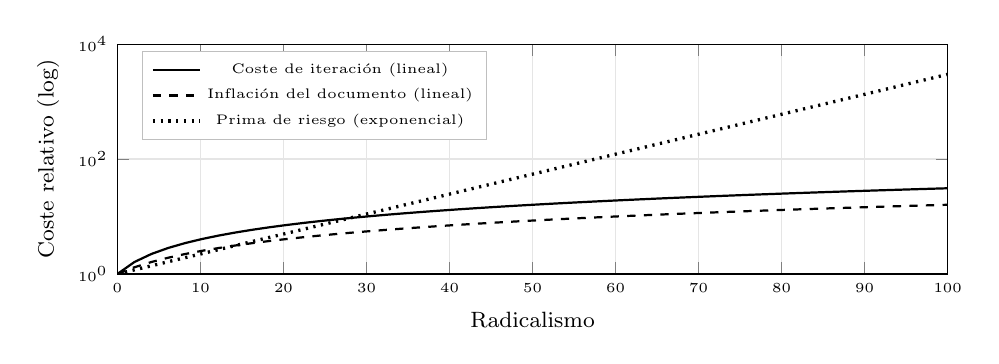
\begin{tikzpicture}
\begin{axis}[
    width=\columnwidth,
    height=4.5cm,
    xlabel={\footnotesize Radicalismo},
    ylabel={\footnotesize Coste relativo (log)},
    ymode=log,
    xmin=0, xmax=100,
    ymin=1, ymax=10000,
    grid=major,
    grid style={gray!20},
    legend style={at={(0.03,0.97)},anchor=north west,font=\tiny,draw=gray!50},
    tick label style={font=\tiny},
    label style={font=\footnotesize},
]
\addplot[black, thick, domain=0:100, samples=50] {1 + 0.3*x};
\addlegendentry{Coste de iteración (lineal)}
\addplot[black, thick, dashed, domain=0:100, samples=50] {1 + 0.15*x};
\addlegendentry{Inflación del documento (lineal)}
\addplot[black, thick, dotted, line width=1.2pt, domain=0:100, samples=100] {exp(0.08*x)};
\addlegendentry{Prima de riesgo (exponencial)}
\end{axis}
\end{tikzpicture}
\caption{Escalada de costes a través de tres canales. La prima de riesgo domina en niveles altos de radicalismo.}
\label{fig:radicalism}
\end{figure}

Fundamentalmente, esto no es censura. Ninguna afirmación se prohíbe. El sistema pone precio al riesgo (Tabla~\ref{tab:costs}).

\begin{table}[ht]
\centering
\caption{Comparación de costes según el tipo de afirmación.}
\label{tab:costs}
\footnotesize
\begin{tabular}{@{}lcccc@{}}
\toprule
\textbf{Tipo} & \textbf{Iter.} & \textbf{Doc} & \textbf{Tarifa} & \textbf{Total} \\
\midrule
Creíble & $k_{\min}$ & $B_0$ & $P_{\min}$ & Bajo \\
Controvertida & $k_{\text{med}}$ & $B_0{+}k\Delta$ & $\alpha e^{\beta d}$ & Moderado \\
Radical & $k_{\max}$ & $\gg B_0$ & $\gg P_{\min}$ & Muy alto \\
Fraudulenta & $\to\infty$ & --- & --- & Impublicable \\
\bottomrule
\end{tabular}
\end{table}

% ============================================================
% 6. REPUTATION AND RISK
% ============================================================
\section{Reputación y evaluación del riesgo}

\subsection{Modelo de acumulación de reputación}

La reputación exhibe tres propiedades: \textbf{acumulación lenta} (crecimiento incremental mediante comportamiento consistente), \textbf{destrucción rápida} (un solo fraude puede reducir la puntuación de forma catastrófica) y \textbf{evaluación individual} (cada parte consumidora puede aplicar su propia función de agregación).

\subsection{Autoridades Reputables}

Una Autoridad Reputable revisa las afirmaciones y, si queda satisfecha, las cofirma---arriesgando su propia reputación (Fig.~\ref{fig:authority}). La asimetría es intencionada: ganar reputación es lento (incremental $+\delta$ por cada respaldo honesto), mientras que perderla es catastrófico ($-\Delta \gg \delta$ por cada respaldo falso; a modo ilustrativo, p.\ ej., $+2\%$ frente a $-70\%$). La estrategia óptima es siempre rechazar las afirmaciones sospechosas. Los valores concretos de $\delta$ y $\Delta$ son parámetros del sistema.

\begin{figure}[ht]
\centering
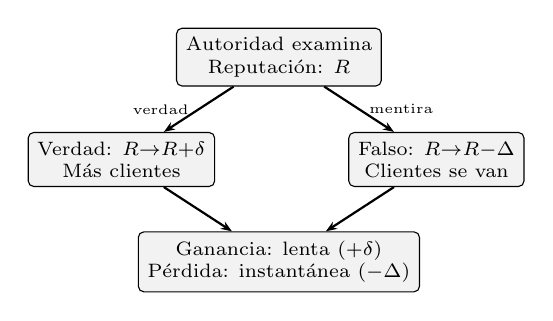
\begin{tikzpicture}[
    box/.style={draw, rounded corners=2pt, minimum width=2cm, minimum height=0.6cm, align=center, font=\scriptsize, fill=black!5},
    arr/.style={-{Stealth[length=4pt]}, thick}
]
\node[box] (exam) at (0,0) {Autoridad examina\\Reputación: $R$};
\node[box] (true) at (-2,-1.3) {Verdad: $R{\to}R{+}\delta$\\Más clientes};
\node[box] (false) at (2,-1.3) {Falso: $R{\to}R{-}\Delta$\\Clientes se van};
\node[box] (insight) at (0,-2.6) {Ganancia: lenta ($+\delta$)\\Pérdida: instantánea ($-\Delta$)};

\draw[arr] (exam) -- node[left,font=\tiny] {verdad} (true);
\draw[arr] (exam) -- node[right,font=\tiny] {mentira} (false);
\draw[arr] (true) -- (insight);
\draw[arr] (false) -- (insight);
\end{tikzpicture}
\caption{Autoridad Reputable---incentivos asimétricos.}
\label{fig:authority}
\end{figure}

\subsection{Reputación multidimensional}

La reputación no es un escalar sino un vector a lo largo de múltiples dimensiones: fiabilidad financiera, integridad personal, competencia profesional, compromiso cívico y otras (Fig.~\ref{fig:reputation-radar}). Distintos proveedores de evaluación proyectan este vector de manera diferente según el contexto---un prestamista prioriza la fiabilidad financiera, un empleador la competencia profesional, un vecino el comportamiento cívico. No existe una única puntuación de reputación ``correcta''; solo perspectivas.

\begin{figure}[ht]
\centering
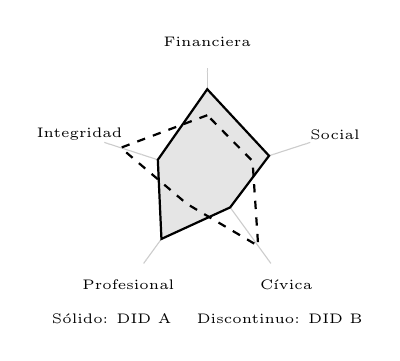
\begin{tikzpicture}[scale=0.55]
\foreach \a/\l in {90/Financiera,162/Integridad,234/Profesional,306/Cívica,18/Social} {
  \draw[gray!40] (0,0) -- (\a:2.5);
  \node[font=\tiny, align=center] at (\a:3.1) {\l};
  \foreach \r in {0.8,1.6,2.4} {
    \fill[black!15] (\a:\r) circle (0.5pt);
  }
}
\draw[thick, fill=black!10] (90:2.0) -- (162:1.2) -- (234:1.8) -- (306:0.9) -- (18:1.5) -- cycle;
\draw[thick, dashed] (90:1.4) -- (162:2.1) -- (234:0.8) -- (306:2.0) -- (18:1.1) -- cycle;
\node[font=\tiny] at (0,-3.3) {Sólido: DID A \quad Discontinuo: DID B};
\end{tikzpicture}
\caption{Vectores de reputación multidimensionales. Distintos DID exhiben perfiles diferentes en las dimensiones.}
\label{fig:reputation-radar}
\end{figure}

\subsection{Evaluación de riesgo democratizada}

La RSN democratiza la evaluación sistemática del riesgo---una capacidad actualmente concentrada en las instituciones financieras pero aplicable mucho más allá de la banca. Conglomerados industriales que evalúan la fiabilidad de sus proveedores, aseguradoras que ponen precio al riesgo conductual, la debida diligencia en fusiones y adquisiciones, la estimación de la vida útil de equipos en la industria---dondequiera que el riesgo de la contraparte requiera evaluación, la RSN ofrece una alternativa descentralizada e impulsada por el mercado. Un mercado de servicios de interpretación traduce los datos brutos de reputación multidimensional en resúmenes accionables, haciendo que la evaluación de la contraparte sea accesible para cualquier participante a un coste marginal.

% ============================================================
% 7. CONSENSUS AND DISPUTE RESOLUTION
% ============================================================
\section{Consenso y resolución de disputas}

\subsection{Modelo de justicia descentralizada}

La RSN replantea la justicia como un problema de negociación bilateral. La amenaza de un daño reputacional permanente y verificable es un elemento disuasorio más eficaz que un proceso judicial que la parte perjudicada no puede permitirse.

\subsection{Consenso emergente}

Cada participante mantiene un umbral personal de satisfacción. El consenso agregado de la red emerge como el promedio estadístico de miles de negociaciones bilaterales (Fig.~\ref{fig:consensus}). Una respuesta muy por encima del consenso (bárbara) es cara de publicar. Una respuesta cercana al consenso (proporcional) es barata. El consenso no es una regla---es una señal de precio.

\begin{figure}[ht]
\centering
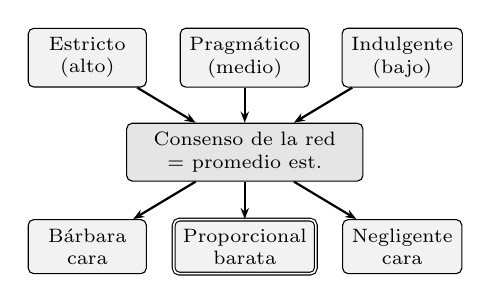
\begin{tikzpicture}[
    person/.style={draw, rounded corners=2pt, minimum width=1.5cm, minimum height=0.5cm, align=center, font=\scriptsize, fill=black!5},
    arr/.style={-{Stealth[length=4pt]}, thick}
]
\node[person] (a) at (-2,0) {Estricto\\(alto)};
\node[person] (b) at (0,0) {Pragmático\\(medio)};
\node[person] (c) at (2,0) {Indulgente\\(bajo)};
\node[person, fill=black!10, minimum width=3cm] (cons) at (0,-1.2) {Consenso de la red\\= promedio est.};
\node[person] (exp) at (-2,-2.4) {Bárbara\\cara};
\node[person, double] (prop) at (0,-2.4) {Proporcional\\barata};
\node[person] (neg) at (2,-2.4) {Negligente\\cara};

\draw[arr] (a) -- (cons);
\draw[arr] (b) -- (cons);
\draw[arr] (c) -- (cons);
\draw[arr] (cons) -- (exp);
\draw[arr] (cons) -- (prop);
\draw[arr] (cons) -- (neg);
\end{tikzpicture}
\caption{Consenso emergente a partir de umbrales de satisfacción individuales.}
\label{fig:consensus}
\end{figure}

\subsection{Calibración del castigo}

Cada Titular de un DID declara públicamente sus respuestas a categorías específicas de mala conducta. Las declaraciones desproporcionadamente severas o indulgentes atraen señales de reputación negativas. Las declaraciones proporcionales se aceptan sin fricción---un sistema de castigo autocalibrado.

Las declaraciones de consenso están sujetas ellas mismas a la detección de hipocresía: comprometerse declarativamente con una posición de consenso mientras se actúa de forma incoherente constituye una infracción reputacional más grave que la desviación subyacente, ya que demuestra un engaño intencionado.

\subsection{Delegación}

Todas las actividades dentro de un DID---con una excepción---pueden delegarse en otro DID. \textbf{El rol de Sujeto---el DID sobre cuyo comportamiento trata la afirmación---no puede delegarse; está ligado de forma no transferible al titular de la identidad a quien se refiere la afirmación.} Los demás roles activos---Emisor, Autoridad, Testigo, Verificador---pueden transferirse a un DID delegado designado, ya sea para verificación, envío de afirmaciones, participación en el consenso o resolución de disputas. La delegación es revocable en cualquier momento. Esto permite la especialización (por ejemplo, servicios profesionales de verificación) mientras el Titular conserva el control y la responsabilidad últimos. La delegación se aplica a todo el sistema y es esencial para la escalabilidad.

\subsection{De la moral individual al contrato social emergente}

La política declarada de cada DID representa una formalización de la moral individual: lo que el Titular considera aceptable, cómo responde a comportamientos específicos, qué exige de sus contrapartes. Estas políticas no las impone un diseñador del sistema---las elige cada participante y se expresan en forma legible por máquina.

Esta formalización habilita una emergencia en tres etapas. Primero, la moral individual se codifica como \textbf{política}---un conjunto de reglas declaradas, umbrales y funciones de respuesta que el DID se compromete a seguir. Segundo, el agregado de todas las políticas de la red produce una \textbf{ética emergente}---normas estadísticamente observables que ningún participante individual diseñó pero que surgen de la interacción de miles de posiciones morales individuales~\cite{durkheim1893}. Tercero, esta ética emergente, expresada como normas de comportamiento compartidas y ejecutadas mediante señales de precio bilaterales, constituye un \textbf{contrato social medible}---no un constructo teórico que nadie firmó~\cite{rawls1971}, sino un conjunto de reglas empíricamente observable y respaldado por el comportamiento real.

Este proceso refleja los hallazgos de la teoría de los fundamentos morales~\cite{haidt2012}: la moral humana es intuitiva, plural y culturalmente variable. La RSN no requiere el consenso moral como entrada; produce el consenso conductual como salida. El contrato social resultante no es estático---evoluciona a medida que los participantes se unen, se marchan y ajustan sus políticas en respuesta a la retroalimentación de la red. A diferencia de la teoría clásica del contrato social, este contrato es revocable, observable y ejecutable sin un soberano.

% ============================================================
% 8. ECONOMIC MODEL
% ============================================================
\section{Modelo económico}

Las secciones anteriores describieron una herramienta---los mecanismos de verificación de la RSN, su estructura de costes y su consenso emergente. Esta sección describe una metodología para aplicar esa herramienta a la transición fiscal y de gobernanza. La herramienta es de propósito general; la metodología que sigue es una posible aplicación.

\subsection{Estructura de incentivos}

La reputación como capital crea incentivos directos para el comportamiento honesto. En el funcionamiento normal, los participantes construyen reputación de forma natural mediante transacciones cotidianas y compromisos cumplidos. El gasto principal se destina a las afirmaciones \emph{negativas}---registrar el daño causado por otros. Esta asimetría incentiva el comportamiento útil y fiable: ser honesto no cuesta nada adicional, mientras que ser dañino crea un rastro documentado que otros pagarán por preservar. La hipocresía---declarar reglas sin seguirlas---es el modo de fallo más caro, ya que demuestra un engaño intencionado.

\subsection{Sistema fiscal paralelo}

Tres componentes habilitan la presión competitiva: (1)~\textbf{Impuesto Simple}---una única tasa proporcional sin excepciones, inicialmente marginalmente por debajo de la tasa efectiva existente; (2)~\textbf{Registro Electrónico del Gasto (RED)}---invirtiendo el modelo checo EET para que los ciudadanos vigilen el gasto estatal; (3)~\textbf{Asignación Tributaria Dirigida por el Ciudadano}---empezando en un pequeño porcentaje el primer año y alcanzando, tras una década, desde cifras de dos dígitos bajos hasta una migración completa a un sistema dirigido por el ciudadano, según el ritmo de adopción. El tempo real depende de la velocidad a la que surjan alternativas de libre mercado a los servicios estatales y de la disposición del Estado a cooperar con la transición; la función del tiempo no tiene por qué ser lineal, y no hay razón para fijar un límite superior sobre dónde puede acabar llegando la adopción.

% ============================================================
% 9. MIGRATION PATH
% ============================================================
\section{Ruta de migración}

La migración transcurre por tres fases (Fig.~\ref{fig:migration}): \textbf{Fase~1: Superposición} (la RSN como capa informativa, el Estado es el único proveedor), \textbf{Fase~2: Competencia} (la RSN ofrece alternativas funcionales, uso de doble sistema) y \textbf{Fase~3: Transición} (la RSN supera a los equivalentes estatales, migración voluntaria). La transición es reversible en cada etapa.

\begin{figure}[ht]
\centering
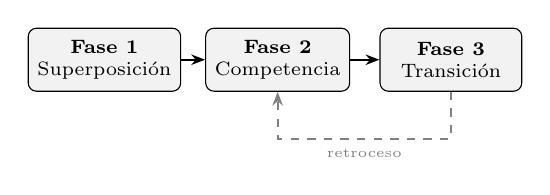
\begin{tikzpicture}[
    phase/.style={draw, rounded corners=3pt, minimum width=1.8cm, minimum height=0.8cm, align=center, font=\scriptsize, fill=black!5},
    arr/.style={-{Stealth[length=5pt]}, thick}
]
\node[phase] (p1) at (0,0) {\textbf{Fase 1}\\Superposición};
\node[phase] (p2) at (2.2,0) {\textbf{Fase 2}\\Competencia};
\node[phase] (p3) at (4.4,0) {\textbf{Fase 3}\\Transición};

\draw[arr] (p1) -- (p2);
\draw[arr] (p2) -- (p3);
\draw[arr, dashed, gray] (p3.south) -- ++(0,-0.6) -| node[below,font=\tiny,pos=0.25] {retroceso} (p2.south);
\end{tikzpicture}
\caption{Migración en tres fases---reversible en cada etapa.}
\label{fig:migration}
\end{figure}

El principal mecanismo de presión es fiscal: cuando los contribuyentes condicionales alcanzan una ``minoría económicamente significativa $X$''---un grupo lo bastante grande como para que la represión contra él cause un daño económico no trivial y la desobediencia civil se convierta en una amenaza creíble---el Estado entra en negociación. A modo ilustrativo, usamos $X \approx 15\%$ del PIB, pero el umbral real depende de la economía concreta.

% ============================================================
% 10. SECURITY ANALYSIS
% ============================================================
\section{Análisis de seguridad}

Consideramos cinco categorías de adversarios: malos actores individuales, grupos organizados, adversarios corporativos, adversarios a nivel estatal y adversarios a nivel de protocolo.

\textbf{Resistencia Sybil}~\cite{douceur2002}. Construir reputación requiere una interacción sostenida y verificable. El coste de un ataque Sybil exitoso escala linealmente con las identidades falsas y cuadráticamente con el nivel de reputación objetivo. Operar múltiples DID en paralelo es posible pero caro por diseño---cada identidad debe acumular reputación de forma independiente mediante actividad genuina. En sociedades libres este coste disuade el abuso casual; en dictaduras, los DID paralelos se convierten en una herramienta de supervivencia que habilita una resistencia compartimentada, la coordinación clandestina y una navegación más segura del mercado negro.

\textbf{Defensa contra la colusión.} Los patrones de respaldo mutuo entre grupos cerrados son detectables mediante el análisis del grafo social. Las funciones de agregación de reputación descuentan las afirmaciones procedentes de fuentes fuertemente agrupadas.

\textbf{Adversario a nivel estatal.} El enrutamiento onion, la ausencia de infraestructura centralizada y la distribución del rol de Verificador entre la base de participantes garantizan que la supresión requiera medidas desproporcionadas frente a cualquier beneficio.

\textbf{Privacidad frente a rendición de cuentas.} La seudonimia---un término medio entre el anonimato y la revelación de identidad---permite a los DID acumular reputación significativa sin revelar la identidad real del Titular.

% ============================================================
% 11. PRIVACY
% ============================================================
\section{Consideraciones sobre la privacidad}

El modelo de privacidad de la RSN se basa en la seudonimia. El Titular controla la revelación de identidad: mínima (seudónimo puro), selectiva (credenciales específicas vinculadas) o total (identidad legal asociada). Las afirmaciones publicadas son permanentes---el sistema admite la corrección contextual pero no el borrado. Un Titular puede abandonar un DID comprometido y empezar de nuevo, renunciando a la reputación acumulada.

% ============================================================
% 12. RELATED WORK
% ============================================================
\section{Trabajo relacionado}

La especificación W3C DID Core~\cite{did2022} y la red Ceramic~\cite{ceramic2023} proporcionan la base de identidad. EigenTrust~\cite{kamvar2003} demostró la agregación distribuida de reputación sin autoridad central. Los SBT~\cite{weyl2022} introdujeron tokens sociales no transferibles. La RSN se diferencia en su énfasis en el coste económico como filtro de calidad y en su mecanismo para poner precio al radicalismo.

Las DAO~\cite{buterin2014} y la votación cuadrática~\cite{buterin2019} demostraron la viabilidad de la gobernanza descentralizada. La RSN deriva el consenso de negociaciones bilaterales de precio en lugar de la votación.

La propuesta se basa en la teoría anarcocapitalista~\cite{rothbard1973,hoppe2001} para la provisión privada de servicios, pero se aparta de ella en dos aspectos críticos: diseña teniendo en cuenta el rencor y los impulsos retributivos en lugar de suponer racionalidad, y propone una transición gradual en lugar de una revolución. El concepto de contratos sociales emergentes tiene antecedentes en la teoría del orden espontáneo de Hayek~\cite{hayek1973}.

\textbf{Anarcoagorismo.} La RSN comparte un terreno común significativo con la contraeconomía agorista~\cite{konkin2006}---en particular el énfasis en construir instituciones paralelas y en el intercambio voluntario. Sin embargo, el agorismo tiende a suponer el interés propio racional como mecanismo de coordinación suficiente y a menudo carece de una ruta de migración concreta desde las estructuras estatales existentes. La RSN incorpora explícitamente tendencias conductuales no racionales y proporciona un mecanismo de presión fiscal para una transición gradual.

\textbf{Meritocracia.} La RSN puede representar una primera descripción funcional de cómo la meritocracia~\cite{young1958} puede emerger como una propiedad sistémica en lugar de un eslogan. Los sistemas meritocráticos tradicionales fracasan porque requieren una autoridad central que defina y haga cumplir el ``mérito''. En la RSN, el mérito emerge de evaluaciones bilaterales: quienes aportan valor acumulan reputación; ningún comité decide quién tiene mérito.

\textbf{La propiedad como privilegio.} La RSN se aparta fundamentalmente de los tratamientos anarcocapitalistas y de la escuela austriaca sobre los derechos de propiedad como naturales y absolutos. En el marco de la RSN, la propiedad es un \emph{privilegio}---un reconocimiento social que, en casos extremos, puede ser retirado por la comunidad cuando un participante viola fundamentalmente las normas compartidas (traición, negativa a defender a la comunidad en una crisis existencial, explotación sistemática). Esto no es una expropiación estatal, sino la retirada del reconocimiento social por parte de la red de relaciones bilaterales.

% ============================================================
% 13. LIMITATIONS
% ============================================================
\section{Discusión y limitaciones}

\textbf{Arranque en frío.} El valor de la RSN depende de los efectos de red; los adoptantes tempranos afrontan un valor limitado hasta que la participación alcanza un umbral. Sin embargo, incluso desde etapas iniciales, la red DID sirve como una fuente de información complementaria útil. Se espera que la evaluación temprana de la reputación y la valoración de las autoridades se desarrollen gradualmente con una sofisticación creciente.

\textbf{Anti-parasitismo y control de acceso.} Los DID objetivo pueden imponer tarifas graduadas y restricciones de acceso a las consultas de DID de baja reputación. Esto no es binario sino una escala continua: cuanta menos reputación tiene un DID que consulta, menos información recibe, más espera y más paga. Este mecanismo incentiva la participación genuina por encima del consumo pasivo.

\textbf{Desigualdad de acceso.} El coste de publicar afirmaciones puede filtrar reclamaciones legítimas de participantes económicamente desfavorecidos. Mitigación: cada participante actúa simultáneamente como verificador potencial (o delega este rol) y gana tarifas de verificación. En un horizonte temporal suficiente, un participante no radical debería aproximarse a la neutralidad financiera---los ingresos por verificación compensando aproximadamente los costes de publicación. Esto es una expectativa estadística, no una garantía.

\textbf{Desigualdad de reputación.} Los adoptantes tempranos acumulan ventajas que pueden crear barreras para los que llegan más tarde. Sin embargo, la evaluación de la reputación la realizan proveedores externos que pueden optar por mitigar la ventaja del primer participante mediante sus algoritmos de agregación. Ser el primero con una buena reputación es una ventaja económica comparativa legítima---y eso es intencionado.

\textbf{Cuestiones abiertas.} Las funciones de coste óptimas, los estándares de agregación, la gobernanza del protocolo y la interacción con datos de reputación sintética generados por IA siguen siendo áreas para trabajo futuro.

Este artículo no afirma que la RSN vaya a producir resultados óptimos en todas las circunstancias. Afirma que la RSN representa una alternativa \emph{viable}---técnicamente implementable, económicamente autosostenible y socialmente compatible con las tendencias conductuales humanas tal como son en realidad.

% ============================================================
% 14. CONCLUSION
% ============================================================
\section{Conclusión}

Este artículo ha presentado la Red Social de Reputación, un protocolo descentralizado que habilita el intercambio de reputación seudónimo y verificable. El Principio del Radicalismo Costoso garantiza que las afirmaciones fraudulentas queden fuera de precio sin necesidad de censura. La ruta de migración propuesta permite una transición gradual y reversible desde las instituciones existentes. El diseño incorpora la naturaleza humana tal como es---incluidas la mezquindad, el rencor y el deseo de satisfacción retributiva---en lugar de exigir una transformación ideológica. El resultado no es una utopía, sino un sistema en el que la justicia es accesible, la reputación se gana y el coste de la mala conducta lo soporta la parte que lo causó.

% ============================================================
% REFERENCES
% ============================================================
\bibliography{references}

\end{document}
